\documentclass[12pt]{article}
\usepackage[a4paper, total={7.5in, 10.7in}]{geometry}
\usepackage{array}
\usepackage{graphicx, subfig, wrapfig, fancyhdr, lastpage, multicol ,color,arydshln,makecell, mhchem}

\newcommand\headerMe[2]{\noindent{}#1\hfill#2}
\usepackage[mathscr]{euscript}
\usepackage{tabularray}

\setlength{\columnseprule}{1pt}
\def\columnseprulecolor{\color{blue}}


\pagestyle{fancy}
\fancyhf{}

\cfoot{ \vspace{-0.8cm}\em{Page \thepage \hspace{1pt} / \pageref{LastPage}}}
\begin{document}

\headerMe{Royaume du Maroc}{année scolaire \emph{2024-2025}}\\
\headerMe{Ministère de l'Éducation nationale, }{  Professeur :\emph{Zakaria Haouzan}}\\
\headerMe{du Préscolaire et des Sports}{Établissement : \emph{Lycée SKHOR qualifiant}}\\
\vspace{-1cm}
\begin{center}
Devoir Surveillé  N°4 - S1 \\
    2ème année baccalauréat Sciences Mathématiques\\
Durée 4h00
\\
    \vspace{-.2cm}
\hrulefill
\Large{Chimie 7pts - 63min}
\hrulefill\\

    \emph{Les deux parties sont indépendantes}
\end{center}
%end Headerss------------------------
%__________________Chimie ______________________-
%%%%%%%+_+_+_+_+_+_+_+_+_Partie1

 \section*{Partie 1 : Etude d’une solution aqueuse d’acide méthanoïque\dotfill(3,5pt) }
%\begin{wrapfigure}{r}{0.16\textwidth}
	%\vspace{-1.2cm}
%%\begin{center}
  %%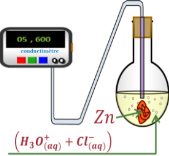
\includegraphics[width=0.16\textwidth]{./img/chimie01.png}
%%\end{center}
%\end{wrapfigure}


%\begin{wrapfigure}[12]{r}{0.38\textwidth}
	%\vspace{-2.4cm}
%\begin{center}
  %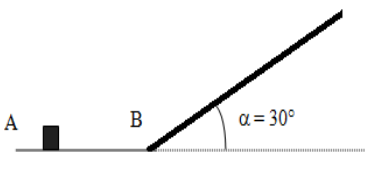
\includegraphics[width=0.38\textwidth]{./img/img00.png}
%\end{center}
%\end{wrapfigure}

\emph{L’acide méthanoïque ou acide formique est une substance naturelle secrétée par les fourmis et les abeilles
pour se défendre contre les prédateurs, sa première isolation a été réalisée par distillation des corps de
fourmis.}

\begin{wrapfigure}[9]{r}{0.35\textwidth}
  \begin{center}
	  \vspace{-1cm}
	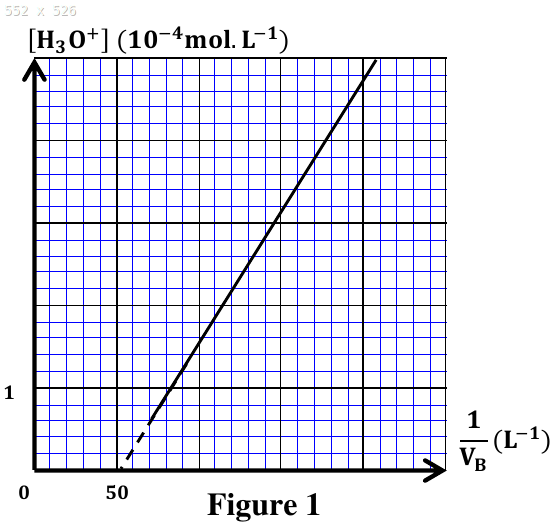
\includegraphics[width=0.4\textwidth]{./img/chimie_fig.png}
  \end{center}
\end{wrapfigure}

Le but de cette partie et de vérifier par dosage le pourcentage massique de l’acide méthanoïque dans une
solution commerciale, et d’étudier sa solution aqueuse.
Dans les conditions ordinaires, l’acide méthanoïque est à l’état liquide.
L’étiquette du flacon d’une solution commerciale $(S_0)$ de cet acide porte les informations suivantes:
\begin{itemize}
  \item Formule chimique : HCOOH ;
  \item Densité : d =1,15 ;
  \item Le pourcentage massique : p =80\% ;
  \item Masse volumique de l’eau : $\rho_e =1kg.L^{-1}$
\end{itemize}

\textbf{Données :}

\begin{itemize}
  \item  p =80\% signifie que 100g de solution commerciale contient 80 g d’acide pur;
  \item  La masse molaire de l’acide méthanoïque est : $M(HCOOH ) = 46 g.mol^{-1}$ ;
\end{itemize}



\subsection*{1- Vérification par dosage du pourcentage massique:\dotfill}

On prépare une solution aqueuse $(S_A)$ d’acide méthanoïque de concentration molaire $C_A$ et de volume
$V_S =1,0 L$ en ajoutant à l’eau distillée, un volume $V_0 = 2,0 mL$
de la solution commerciale d’acide méthanoïque $(S_0)$ de
concentration molaire $C_0$.

On verse dans un bécher un volume $V_A = 50 mL$ de la solution $(S_A)$ , 
et on dose l’acide méthanoïque par une solution aqueuse $(S_B)$ d’hydroxyde de sodium $({Na^{+}}_{(aq)} + {HO^{-}}_{(aq)})$
 de concentration  molaire $C_B = 0,10 mol.L^{-1}$ . Les résultats de mesure du pH en
fonction du volume $V_B$ d’hydroxyde de sodium versé ont permis
de tracer la courbe exprimant la variation de la concentration des
ions oxonium dans le mélange réactionnel en fonction de $\frac{1}{V_B}$
 .(figure1)

\begin{tabular}{c : c}
		0,25pt & \makecell[l]{\textbf{1.1. } Ecrire l’équation chimique modélisant la réaction de ce dosage. }\\

			0,75pt & \makecell[l]{\textbf{1.2. } Montrer que la concentration des ions oxonium dans le bécher après l’ajout d’un volume\\ $V_B$ , tel
  que :  $0 < V_B < V_{BE}$ avec $V_{BE}$ le volume de la solution $(S_B)$ versé à l’équivalence, s’écrit :\\
  \\\hspace{3cm}$[H_3O^+] = a.\frac{1}{V_B} + b$ \hspace{1cm}avec $a = K_A.V_{BE}$ et $b=-K_A$\\
  \\
  $K_A$ représente la constante d’acidité du couple $HCOOH/HCOO^-$.}\\

      0,5pt & \makecell[l]{\textbf{1.3. } En exploitant la courbe de la figure 1 déterminer $V_{BE}$ et $K_A$.}\\

      0,5pt & \makecell[l]{\textbf{1.4. } Calculer la concentration $C_A$ de la solution $(S_A)$, et déduire la concentration $C_0$ \\de la solution commerciale}\\


      0,5pt & \makecell[l]{\textbf{1.5. } Vérifier si la valeur du pourcentage massique p est correcte.}\\

	
\end{tabular}
			
\subsection*{2- Etude de la solution (SA) d’acide méthanoïque :\dotfill}

\begin{tabular}{c : c}
		0,25pt & \makecell[l]{\textbf{2.1. } Ecrire l’équation de la réaction de l’acide méthanoïque avec l’eau}\\
    0,75pt & \makecell[l]{\textbf{2.2. } Etablir l’expression de la constante d’acidité K A du couple $HCOOH/HCOO^-$ en fonction \\de $C_A$ et $\tau$ le taux d’avancement final de la réaction, Calculer $\tau$ . Conclure }\\

\end{tabular}


 \section*{Partie 2 : Vérification de la masse de l’acide propanoïque dans un médicament\dotfill(3,5pt) }
\emph{L’acide propanoïque $C_2H_5COOH$ est un liquide que l’on prépare au laboratoire. Il est utilisé comme
agent conservateur et entre dans la composition de certains médicaments et dans la synthèse de certains
arômes.
Cette partie consiste à vérifier, par dosage, la masse de l’acide propanoïque dans un médicament.}

\textbf{Données : } 

\begin{itemize}
  \item Le produit ionique de l’eau: $K_e =10^{-14}$ à 25°C ;
  \item La masse molaire de l’acide propanoïque : $M(C_2H_5COOH) = 74 g.mol^{-1}$.

\end{itemize}


Le médicament étudié est une solution aqueuse notée (S) . Son étiquette descriptive indique la présence
de $46,2 mg$ d’acide propanoïque dans un volume $V = 40 mL$ de cette solution .

Pour vérifier cette indication, on prépare, à 25°C, une solution $(S_A)$ en introduisant dans un bécher un
volume $V_A =10 mL$ de la solution $(S)$ auquel on ajoute $V_e = 50 mL$ d’eau distillée.

On dose l’acide propanoïque présent dans $(S_A)$ à l’aide d’une solution aqueuse $(S_B)$ d’hydroxyde de
sodium ${Na^+}_{(aq)} + {HO^-}_{(aq)}$
 de concentration molaire $C_B = 2,0.10^{-2} mol.L^{-1}$ .
Après l’ajout d’un volume $V_{B1} = 3,9 mL$ de la solution d’hydroxyde de sodium au mélange, la mesure du pH du mélange réactionnel donne la valeur $pH_1=4,86$ .

A l’équivalence, le volume de la solution d’hydroxyde de sodium ajouté est $V_{BE} = 7,8 mL$ .

\vspace{0.5cm}

\begin{tabular}{c : c}
		0,25pt & \makecell[l]{\textbf{1. } Ecrire l’équation modélisant la réaction qui a lieu lors du dosage.}\\

    0,5pt & \makecell[l]{\textbf{2. } Expliquer pourquoi l’ajout du volume $V_e$ d’eau distillée n’influe pas sur la valeur du volume\\ de la solution d’hydroxyde de sodium ajouté à l’équivalence.}\\

0,75pt & \makecell[l]{\textbf{3. } En se basant sur le tableau d’avancement de la réaction du dosage, trouver l’expression du \\taux
d’avancement final de la réaction avant l’équivalence en fonction du pH du milieu \\réactionnel, $K_e$ , $C_B$ ,
$V_A$ , $V_e$ et $V_B$ le volume de la solution d’hydroxyde de sodium ajouté. \\Calculer sa valeur après l’ajout
  de $V_{B1}$ et conclure. }\\

    0,5pt & \makecell[l]{\textbf{4. } Calculer, après l’ajout du volume $VB =V_{B1}$ , les concentrations $[C_2H_5COOH]$ et \\$[C_2H_5COO^-]$. Déduire
la valeur du $pK_A (C_2H_5COOH/C_2H_5COO^-)$ . }\\

		0,5pt & \makecell[l]{\textbf{5. } Justifier la nature basique du mélange réactionnel à l’équivalence. }\\
		0,5pt & \makecell[l]{\textbf{6. } Calculer le pH de la solution (S) }\\
		0,5pt & \makecell[l]{\textbf{7. } Vérifier que la masse de l’acide propanoïque est celle indiquée sur l’étiquette.}\\
\end{tabular}


%\begin{center}
%\begin{tabular}{ |c| c|}
%\hline
%\textbf{Couple acide/base} &\textbf{ Valeur de $pK_A$}\\\hline
	%$HCOOH / HCOO^-$  & 3,75 \\\hline
	%$C_6H_5COOH/C_6H_5COO^-$ &4,2\\\hline
	%$CH_3COOH/CH_3COO^-$&  4,75 \\\hline
	%$CH_3-CH_2-COOH/CH_3-CH_2-COO^-$ &4,9 \\\hline

%\end{tabular}
%\end{center}

%\begin{tabular}{c|l}
	%0,5 & \makecell[l]{\textbf{3. }Déterminer le volume
	%$V_{b1}$ de la solution $S_b$ versée, au cours du dosage, pour que: $\frac{[AH]}{[A^-]} = 2,24$ . }\\
%\end{tabular}

%\hrulefill
%\Large{Physique 13pts/78min}
%\hrulefill\\
\newpage
\begin{center}
    %\vspace{.60cm}
\hrulefill
\Large{Physique 13pts - 75min}
\hrulefill\\
    %\emph{Les  parties sont indépendantes}
\end{center}

%\vspace{-1cm}
\section*{Exercice 2 -Propagation d’une onde mécanique à la surface de l’eau \dotfill(4pts)}

%\begin{wrapfigure}[9]{r}{0.25\textwidth}
  %\begin{center}
	  %\vspace{-1cm}
	%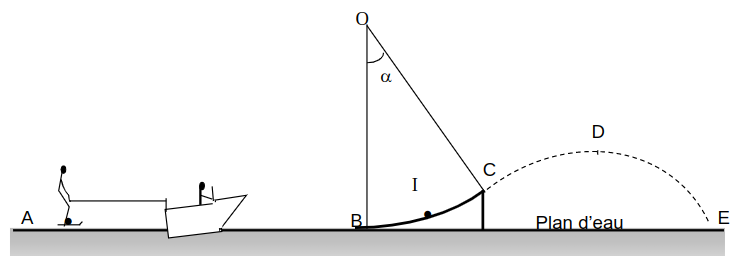
\includegraphics[width=0.19\textwidth]{./img/img01.png}
	%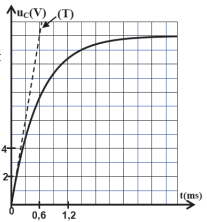
\includegraphics[width=0.25\textwidth]{./img/img02.png}
  %\end{center}
%\end{wrapfigure}

Dans cet exercice, on se propose d’étudier la propagation d’une onde mécanique à la surface de l’eau d’une
piscine et en déduire la profondeur de l’eau.
Une piscine de longueur $L=47,5m$ est constituée de deux parties:

\begin{itemize}
  \item Une partie pour les grands de longueur $L_1 =30m$ et de profondeur $H_1$ (milieu 1);
  \item Une partie pour les petits de longueur $L_2$ et de
profondeur $H_2$ (milieu 2).
\end{itemize}


\begin{center}
	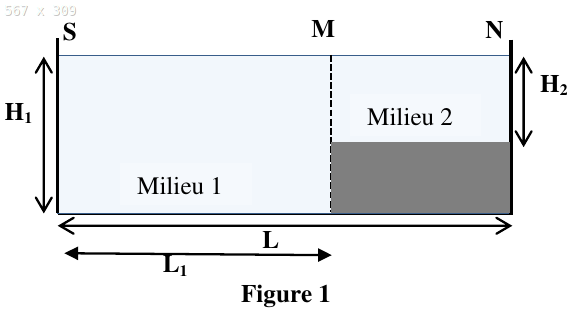
\includegraphics[width=0.45\textwidth]{./img/Onde_00.png}
	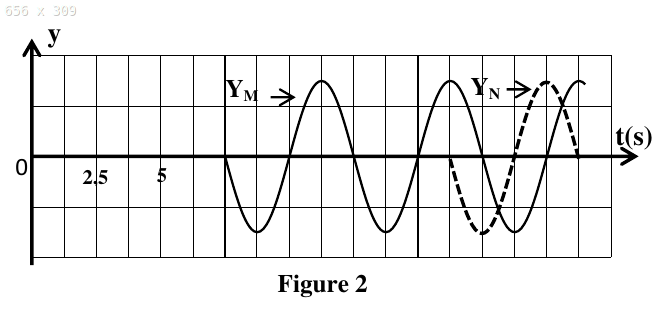
\includegraphics[width=0.45\textwidth]{./img/onde_01.png}
  \end{center}
La figure 1 représente une coupe longitudinale de la piscine contenant les points S , M et N de la surface libre de l’eau.

A un instant de date t=0 , on crée une onde transversale rectiligne sinusoïdale au niveau de S situé au bord de la piscine. On reçoit cette onde à l’aide de deux récepteurs, l’un placé au point M et
l’autre au point N (figure 1).
On néglige l’amortissement et la réflexion des ondes.
Les courbes de la figure 2 représentent les élongations des points M et N en fonction du temps.
La vitesse de propagation de l’onde à la surface de l’eau est donnée par la relation : $v = \sqrt{g.H}$ avec $g=10m.s^{-2}$ l’intensité de pesanteur et H la profondeur de l’eau.


  \vspace{0.5cm}
\begin{tabular}{c|l}
  0,75pt & \makecell[l]{\textbf{1. } Déterminer le retard temporel $\tau_{M/S}$ du mouvement de M par rapport à celui de S
et \\déduire la profondeur $H_1$}\\

	0,75pt & \makecell[l]{\textbf{2. } Calculer la profondeur $H_2$ . }\\
	
	0,5pt & \makecell[l]{\textbf{3. } Calculer les longueurs d’ondes $\lambda_1$ et $\lambda_2$ des ondes respectivement dans le milieu 1\\ et dans le milieu 2.}\\
	
	\end{tabular}

  \vspace{0.4cm}

\begin{wrapfigure}[5]{r}{0.4\textwidth}
  \begin{center}
	  \vspace{-1.6cm}
	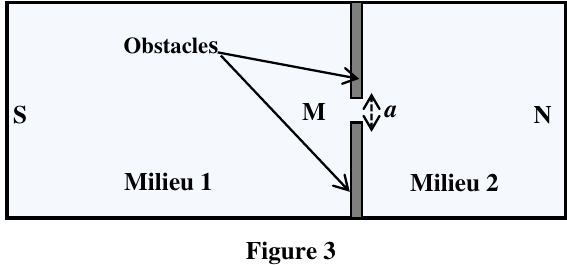
\includegraphics[width=0.4\textwidth]{./img/onde_03.png}
  \end{center}
\end{wrapfigure}


\textbf{4. }Afin d’empêcher les petits de passer chez les grands, deux obstacles ont été placés au niveau du point M et séparés d’une distance a telle que $a \ll \lambda_1$ .La figure 3 représente une vue de dessus de la piscine.



\begin{tabular}{c|l}

0,25pt  & \makecell[l]{\textbf{4.1. }  Donner le nom du phénomène qui se \\produit lors
du passage de l’onde entre les deux obstacles.}\\

 0.5pt& \makecell[l]{\textbf{4.2. }  Reproduire la figure 3 et y représenter, \\(en utilisant l’échelle: $1cm \leftrightarrow 10m$ , trois lignes de crêtes de
l’onde dans chaque milieu.}\\

	\end{tabular}


  \vspace{0.3cm}
\hspace{-1cm}\textbf{5- Propagation de la lumière dans deux milieux différents  \dotfill(1,25pts)}

On place un prisme en verre équilatéral sur un miroir plan. Un rayon lumineux jaune arrive sur le miroir au point I sous un angle d'incidence i = 75°, puis frappe le prisme au point J pour se propager à l'intérieur parallèlement au miroir, comme le montre la figure ci-dessous :

  \begin{center}
	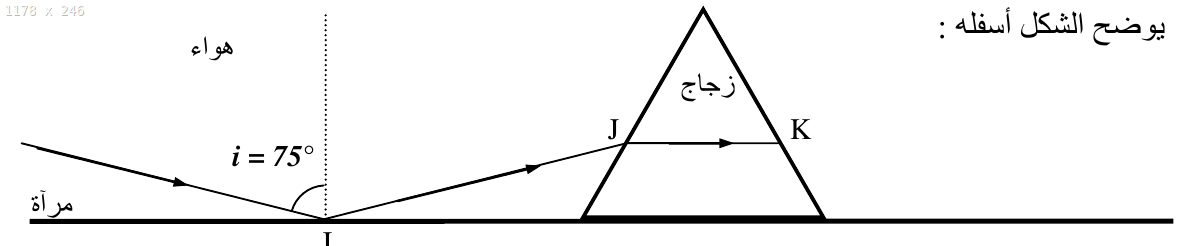
\includegraphics[width=0.8\textwidth]{./img/Onde_02.png}
  \end{center}
\begin{tabular}{c|l}	

  0,25 & \makecell[l]{\textbf{5.1 } Trouvez l'indice de réfraction du verre pour la lumière jaune $n_{jaune}$.}\\
	0,25 & \makecell[l]{\textbf{5.2 } Calculez l'angle d'incidence lorsque le rayon lumineux frappe à nouveau le miroir au point L \\après avoir émergé du prisme au point K.}\\
	0,5 & \makecell[l]{\textbf{5.3 } Sachant que l'indice de réfraction d'un milieu diminue légèrement quand la longueur d'onde \\de la lumière qui s'y propage augmente, décrivez qualitativement comment se propagent la lumière \\rouge et la lumière bleue dans les mêmes conditions expérimentales.}\\
	0,25 & \makecell[l]{\textbf{5.4 } Qu'observera-t-on aux points I et L dans le cas de l'incidence d'une lumière blanche dans \\les mêmes conditions expérimentales ?}\\
	
\end{tabular}




\section*{Exercice 3-  Datation par le couple rubidium-strontium \dotfill(2,5 pts)}

La méthode de datation par le couple rubidium-strontium est une technique de datation de formation des roches, basée sur la mesure des proportions des éléments rubidium et strontium dans différents minéraux (Feldspath, Mica\ldots) de ces roches, sans avoir besoin de connaître les quantités de matière initiales des éléments rubidium et strontium.

Le rubidium $\ce{^{87}_{37}Rb}$ est un isotope radioactif, qui se désintègre en strontium $\ce{^{87}_{38}Sr}$ avec émission d'une particule $\ce{^{A}_{Z}X}$.

\textbf{Données :}
\begin{itemize}
\item La constante radioactive du rubidium 87 est : $\lambda = 1,42\cdot10^{-11}\ \text{an}^{-1}$
\item Les masses :
  \begin{itemize}
  \item $m(\ce{^{87}_{37}Rb}) = 86,8888823\ \text{u}$ \hspace{1.5cm} $m(\ce{^{87}_{38}Sr}) = 86,8880307\ \text{u}$
  \item $m(\ce{^{A}_{Z}X}) = 0,0005486\ \text{u}$  \hspace{1.5cm} $1\ \text{u} = 931,5\ \text{MeV}/c^2$
  \end{itemize}
\end{itemize}


\begin{tabular}{c|l}	

	0,5pt  & \makecell[l]{\textbf{1. } Écrire l'équation de désintégration de $\ce{^{87}_{37}Rb}$ et déduire son type.}\\
	0,5pt & \makecell[l]{\textbf{2. } Calculer, en MeV, $\Delta E$ l'énergie libérée par la désintégration d'un noyau de $\ce{^{87}_{37}Rb}$.}\\
	
\end{tabular}

\textbf{3. }Le minéral d'une roche granitique, emprisonne lors de sa formation une quantité de rubidium radioactif $\ce{^{87}_{37}Rb}$ et une quantité de strontium constituée des isotopes stables $\ce{^{87}_{38}Sr}$ et $\ce{^{86}_{38}Sr}$.

On désigne par :
\begin{itemize}
\item $t_0 = 0$ : l'instant de formation de la roche et de ses minéraux
\item $N_0(\ce{^{87}_{37}Rb})$ le nombre de noyaux de rubidium 87 et $N_0(\ce{^{87}_{38}Sr})$ le nombre de noyaux de strontium 87 présents dans le minéral de la roche à l'instant $t_0$
\item $N(\ce{^{87}_{37}Rb})$ le nombre de noyaux de rubidium 87 et $N(\ce{^{87}_{38}Sr})$ le nombre de noyaux de strontium 87 qui sont présents dans le même minéral à l'instant $t$
\item $N(\ce{^{86}_{38}Sr})$ le nombre de noyaux de strontium 86 présents dans ce minéral
\end{itemize}

On note $u$ et $v$ les rapports à un instant $t$ :
$u = \frac{N(\ce{^{87}_{37}Rb})}{N(\ce{^{86}_{38}Sr})}$ et $v = \frac{N(\ce{^{87}_{38}Sr})}{N(\ce{^{86}_{38}Sr})}$


	\begin{tabular}{c|l}	
	0,5pt & \makecell[l]{\textbf{3.1. } Montrer que le nombre de noyaux de strontium 87 présents dans le minéral à l'instant $t$ \\s'écrit :\\
$N(\ce{^{87}_{38}Sr}) = N(\ce{^{87}_{37}Rb})(e^{\lambda t}-1) + N_0(\ce{^{87}_{38}Sr})$}\\ 
	0,25pt & \makecell[l]{\textbf{3.2. } Déduire que : $v = au + b$, avec $a = (e^{\lambda t}-1)$ et $b = \frac{N_0(\ce{^{87}_{38}Sr})}{N(\ce{^{86}_{38}Sr})}$}\\ 
	\end{tabular}

\begin{wrapfigure}[2]{r}{0.3\textwidth}
  \begin{center}
	  \vspace{-1.2cm}
	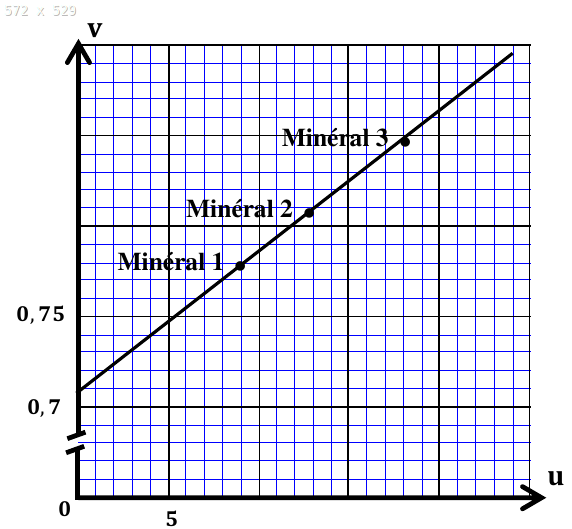
\includegraphics[width=0.3\textwidth]{./img/nuc00.png}
  \end{center}
\end{wrapfigure}

  \textbf{4. }La mesure expérimentale des rapports $u$ et $v$ à la même date pour trois minéraux différents emprisonnés dans la roche a permis d'obtenir une courbe.

	\begin{tabular}{c|l}	
	0,5pt & \makecell[l]{\textbf{4.1. } Déterminer $t_a$ l'âge approximatif de la roche.}\\ 
	0,25pt & \makecell[l]{\textbf{4.2. } Pourquoi n'a-t-on pas utilisé le carbone 14 de demi-vie \\5730 ans pour dater cette roche ?}\\ 
	\end{tabular}

  \vspace{1cm}

\section*{Exercice 4: Electricité- Le Voltmètre Numérique . \dotfill(1,75pts)}

\emph{Ces dernières années, le voltmètre numérique a trouvé sa place parmi les instruments de laboratoire utilisés pendant les séances pratiques. Nous savons tous que cet appareil est utilisé pour mesurer la tension. Cependant, ce que nous ne savons pas, c'est que cet appareil ne mesure pas la tension directement, mais après un certain nombre d'impulsions. Le voltmètre contient une horloge qui émet des impulsions périodiques dont la période $T_0$ est très petite et fixée par le fabricant.}

 L'objectif de cet exercice est de comprendre le principe de mesure d'une tension continue à l'aide d'un voltmètre numérique qui comprend essentiellement un circuit électrique contenant un interrupteur K à trois positions,relié à un compteur(non représenté sur la figure) et un conducteur ohmique de résistance R (également non représenté sur la figure).

À l'instant que nous considérons comme origine des temps $t_0 = 0s$, le condensateur est déchargé.


\begin{center}
	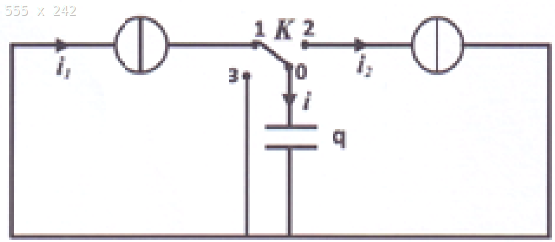
\includegraphics[width=0.3\textwidth]{./img/capcity00.png}
  \end{center}

  Pendant une durée $t_1$, qui est imposée par le fabricant et dont la valeur est un multiple entier de la période de l'horloge $T_0$, soit $t_1 = n_0·T_0$, l'interrupteur K est en position (1), chargeant alors un condensateur de capacité C.

  Pendant $t_1$ constant, le courant de charge $i_1$ est proportionnel à la tension continue U à mesurer, où : $i_1 = \frac{U}{R}$.\\

\begin{tabular}{c|l}	

  0,5pt  & \makecell[l]{\textbf{1.}Donnez l'expression de la charge $q_1$ du condensateur à l'instant $t_1$ en fonction de R, U, $n_0$ \\et $T_0$. }\\
\end{tabular}

\textbf{2. }Après cette durée $(t_1)$, l'interrupteur revient en position $(2)$ : le condensateur se décharge jusqu'à ce que sa charge devienne nulle.

Durant cette phase, l'intensité du courant de décharge $i_2$ est proportionnelle à une tension de référence Uréf (par exemple 2000 V dans le cas d'un calibre 2V), où : $i_2 = \frac{U_{ref}}{R}$.

Entre ces deux instants ($t_1$ et $t_2$), le compteur compte le nombre n d'impulsions émises par l'horloge où : $t_2 - t_1 = n·T_0$.

Ce cycle se répète à nouveau à partir d'un instant $t_3 = 2t_1$, et entre les deux instants dont les dates sont $t_2$ et $t_3$, l'interrupteur K est revenu en position (3) où le condensateur reste déchargé.


\begin{tabular}{c|l}	

  0,25pt  & \makecell[l]{\textbf{2.1. } Tracez l'allure de la courbe de tension $u_c$ aux bornes du condensateur entre les instants\\ $t = t_0 = 0s$ et $t = t_4$.  }\\
  0,25pt  & \makecell[l]{\textbf{2.2. } Donnez l'expression de la variation de la charge du condensateur entre les instants \\$t_1$ et $t_2$ en fonction de : R, Uréf, n et $T_0$. }\\
  0,25pt  & \makecell[l]{\textbf{2.3. }  Déduisez l'expression de la tension U en fonction de : Uréf, n et $n_0$. }\\
  0,25pt  & \makecell[l]{\textbf{2.4. } Comparez n et $n_0$.}\\
  0,25pt  & \makecell[l]{\textbf{2.5. } Pourquoi la mesure de tension avec cet appareil est-elle considérée \\comme une mesure de temps ?}\\
\end{tabular}



\section*{Exercice 5 – Electricité –  Réponse d'un dipôle RL à un échelon de tension\dotfill(1,25pts)}

\begin{wrapfigure}[2]{r}{0.2\textwidth}
  \begin{center}
	  \vspace{-1.2cm}
	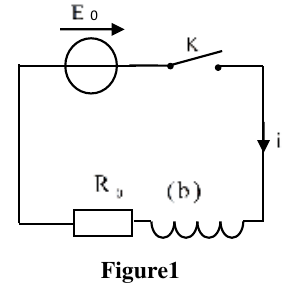
\includegraphics[width=0.2\textwidth]{./img/RL_00.png}
  \end{center}
\end{wrapfigure}


On réalise le montage du circuit électrique comportant :
\begin{itemize}
\item Un générateur de tension de force électromotrice $E_0$
\item Un conducteur ohmique de résistance $R_0$
\item Une bobine (b) d'inductance L et de résistance r
\item Un interrupteur K
\end{itemize}

On ferme l'interrupteur K à un instant pris comme origine des dates (t = 0).


\begin{center}
	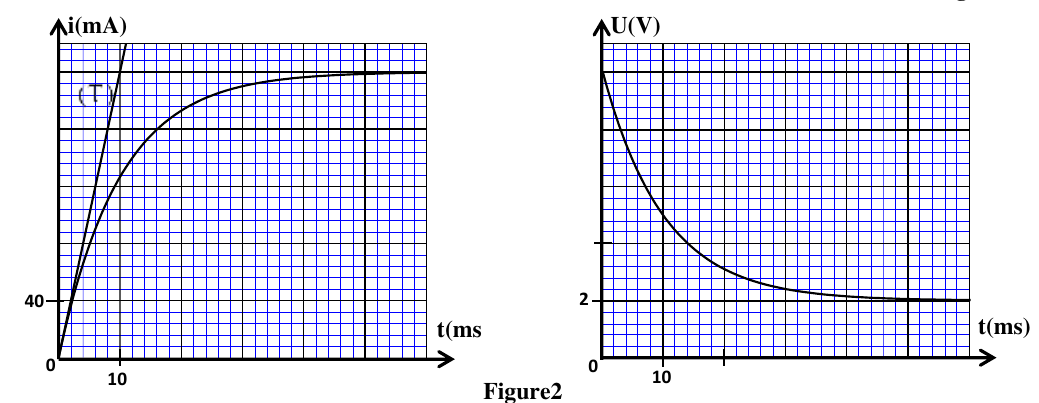
\includegraphics[width=1\textwidth]{./img/RL_01.png}
  \end{center}


\begin{tabular}{c|l}	

	0,25pt & \makecell[l]{\textbf{1. } Établir l'équation différentielle vérifiée par i(t).}\\
	0,25pt & \makecell[l]{\textbf{2. } Déterminer graphiquement la valeur de $E_0$.}\\
	 0,25pt & \makecell[l]{\textbf{3. }Montrer que $L = 0,5\ \text{H}$.}\\
	 0,5pt& \makecell[l]{\textbf{4. } Déterminer la valeur de r et celle de $R_0$.}\\
\end{tabular}


\section*{Exercice 6 – Electricité –  Étude des oscillations dans un circuit RLC série\dotfill(1,25pts)}


\begin{wrapfigure}[2]{r}{0.2\textwidth}
  \begin{center}
	  \vspace{-1.2cm}
	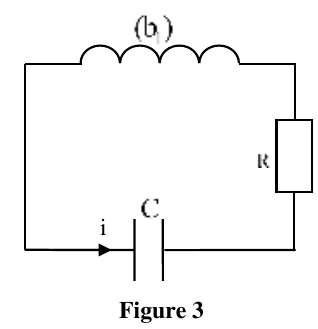
\includegraphics[width=0.2\textwidth]{./img/RLC_00.png}
  \end{center}
\end{wrapfigure}


\textbf{1. } Oscillations libres dans le circuit RLC

On monte en série, à la date t = 0 :

\begin{itemize}
\item Un condensateur de capacité C initialement chargé
\item Une bobine $(b_1)$ d'inductance $L_1 = 0,5\ \text{H}$ et de résistance négligeable
\item Un conducteur ohmique de résistance $R = 150\ \Omega$
\end{itemize}


\begin{center}
	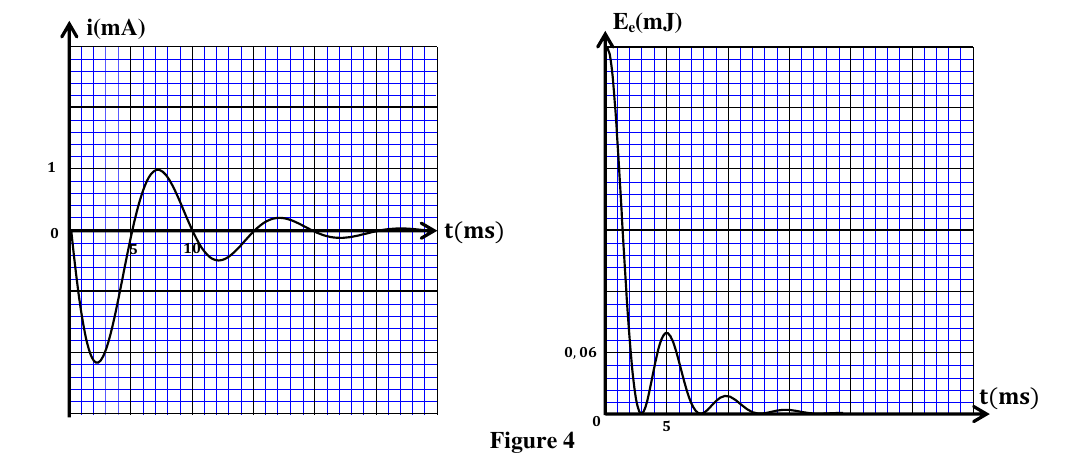
\includegraphics[width=1\textwidth]{./img/RLC_01.png}
  \end{center}


\begin{tabular}{c|l}	

	0,25pt & \makecell[l]{\textbf{1.1. } En considérant la pseudo-période égale à la période propre de l'oscillateur, trouver la \\valeur de la capacité C du condensateur. On prend $\pi^2 = 10$.}\\
		0,5pt & \makecell[l]{\textbf{2.2. } Soit $E_t$ l'énergie totale du circuit à un instant t. Exprimer $\frac{dE_t}{dt}$ en fonction de R et i. \\Conclure.
}\\
		0,5pt & \makecell[l]{\textbf{2.3. } Trouver $\Delta E_t$ l'énergie dissipée par effet Joule dans le circuit entre \\les instants t = 0 et t = 4 ms.
}\\

\end{tabular}


\section*{Exercice 7 – Electricité –   Couplage de deux circuits L//C \dotfill(1,5pts)}

On considère les deux circuits oscillants (LC) identiques
couplés par un condensateur de capacité $C'$ . Lorsqu’on
ferme l’interrupteur à t = 0 il n’y a aucun courant dans
le circuit.

\begin{center}
	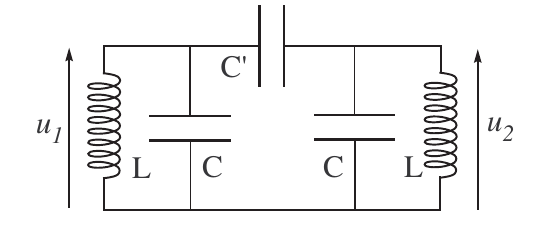
\includegraphics[width=0.6\textwidth]{./img/lcpara.png}
  \end{center}


\begin{tabular}{c|l}	

	0,5pt & \makecell[l]{\textbf{1. } Déterminer les équations différentielles vérifiées par $u_1(t)$ et $u_2(t)$.}\\
  0,5pt & \makecell[l]{\textbf{2. } Établir les équations différentielle vérifiées par $u = u_1 + u_2$ et $v = u_2-u_1$.}\\
	0,5pt & \makecell[l]{\textbf{3. } Quelles conditions initiales de charge des condensateurs permettent d’obtenir \\des $u_1 (t)$ et $u_2 (t)$ non nulles ?}\\

\end{tabular}



	%\vspace{0.5cm}
%\textbf{2. Injection locale d’une solution contenant du rhénium 186.
%Le produit injectable se présente sous la forme d’une solution contenue dans un flacon de volume $V_0= 10 mL$ ayant une activité $a_0 = 4.10^9Bq$ à la date $t=0$, c'est-à-dire à la sortie du laboratoire pharmaceutique.}
	%\begin{tabular}{c|l}

		%1 & \makecell[l]{\textbf{2.1 }Déterminer en jours la valeur de demi-vie $t_{1/2}$ du rhénium $_{75}^{186}Re$}\\

		%0,5 & \makecell[l]{\textbf{2.2 }Trouver, à l’instant $t_1 = 4,8jours$, le nombre $N_1$ de noyau de rhénium contenu dans le flacon.}\\

		%0,5 & \makecell[l]{\textbf{3.2 } À l’instant $t_1$ on prélève du flacon de volume $V_0 = 10mL$ une injection de volume V contenant \\$N = 3,65.10^{13}$ noyaux de rhénium 186, on l’injecte à un malade dans l’articulation de l’épaule, \\trouver la valeur de V.}\\
	%\end{tabular}


%\section*{Partie 2 :  Centrale nucléaire \dotfill(9pts)}
%Dans une centrale nucléaire, les noyaux d'uranium $^{235}_{92}U$ subissent la fission sous le choc d'un neutron
%lent. Un des nombreux processus possibles conduit à la formation d'un noyau de lanthane $^{144}_{57}La$ ,d'un noyau de brome $^{88}_{35}Br$ et  de plusieurs neutrons.

%\begin{tabular}{c|l}

 %1& \makecell[l]{\textbf{1. } Définissez l'énergie de liaison d'un noyau.}\\

 %1 & \makecell[l]{\textbf{2. } Donnez l'expression littérale qui permettra son calcul.}\\

 %1 & \makecell[l]{\textbf{3. } Calculez, en MeV, l'énergie de liaison d’un noyau $^{235}_{92}U$.}\\

 %1 & \makecell[l]{\textbf{4. } Calculez l’énergie de liaison par nucléon de ce noyau.}\\

 %1 & \makecell[l]{\textbf{5. } Ecrivez l’équation de la réaction de fission étudiée.}\\

 %1 & \makecell[l]{\textbf{6. } Exprimez l'énergie libérée par la fission d'un noyau $^{235}_{92}U$ en fonction des énergies de liaison par
%\\ nucléon du noyau père et des noyaux fils et calculez la valeur de cette énergie en MeV.}

 %\end{tabular}

%\textbf{7.  Dans le cœur de la centrale, de nombreuses autres réactions de fission du noyau $^{235}_{92}U$ se produisent. La perte de masse est, en moyenne, de 0,200 u par noyau.}


%\begin{tabular}{c|l}

	%1,5 & \makecell[l]{\textbf{7.1. } Calculez, en MeV, l'énergie moyenne libérée par la fission d’un noyau. Ce résultat est-il \\en concordance avec celui de la question 6 ?}\\

	%1,5 &\makecell[l]{\textbf{7.2. }Calculez, en joule, l'énergie moyenne libérée par une mole de noyaux $^{235}_{92}U$ } 

%\end{tabular}

%\textbf{Données :}
%\begin{itemize}
	%\item Célérité de la lumière dans le vide : $c = 2,998 . 10^8 m.s^{-1}$  
	%\item Masse du noyau d’uranium 235 : $m( ^{235}_{92}U) = 235,0134u$ 

	%\item Energies de liaison par nucléon : $E_l/A(^{144}_{57}La) = 8,28MeV/nucl$éon  ; $E_l/A(^{88}_{35}Br)$=$8,56MeV/nucl$éon
	%\item Constante d'Avogadro : $N_A = 6,02.10^{23} mol^{-1}$
	%\item $1u$ = $1,66055.10^{-27}Kg$ et $1eV = 1,602.10^{-19}J$
	%\item Masse d’un proton : $m(^1_1p) = 1,0073u$ ; Masse d’un neutron $m(^1_0n) = 1,0087u$
%\end{itemize}





\end{document}
